\documentclass[tikz]{standalone}
    \usepackage{tikz}
    \usetikzlibrary{positioning, graphs}
    \usetikzlibrary{graphs.standard}
    \begin{document}
    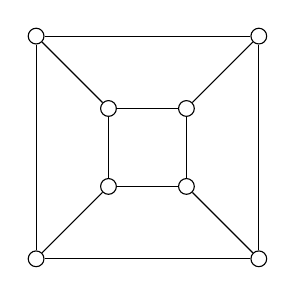
\begin{tikzpicture}
            [every node/.style={draw,circle,inner sep = 0mm, minimum size = 2mm}]
            \graph[clockwise, empty nodes, n = 4, phase=45]{
                subgraph C_n[name = A, radius=.7cm] -- subgraph C_n[name = B, radius=1cm]
            };

    \end{tikzpicture}
    \end{document}